\chapter{Decodificación Manual con GnuPG}

\section{Enunciado:}

\subsection*{5.2.1. Prerrequisitos}

Para realizar este apartado es necesario tener instalada la utilidad \texttt{gnupg}; es un paquete muy común
en distribuciones Linux y en muchas está instalado por defecto.

También puede ser necesaria la utilidad \texttt{ripmime} de utilidades MIME, ya citada en la práctica 1.

\subsection*{5.2.2. Secuencia de operaciones}

Una vez intercambiado el mensaje cifrado y firmado con claves OpenPGP entre compañeros,
hacemos una breve descripción de los pasos necesarios, suponiendo que no se tiene configurado el
uso de GnuPG en nuestro equipo:

\begin{itemize}[label=\textbullet]
    \item Descargar del OpenPGP Key Manager de Thunderbird una copia de nuestra clave privada, protegida
    por contraseña (a un fichero \texttt{claveprivada.asc}).
    \item Descargar también la clave pública del compañero que envió el mensaje (a un fichero \texttt{clave.asc}).
    \item Exportar (guardar como\ldots) el mensaje cifrado y firmado como \texttt{mensaje.eml}.
\end{itemize}

Ahora importamos nuestra clave privada en \texttt{gnupg}:

\begin{itemize}[label=\textbullet]
    \item \texttt{\# gpg --import claveprivada.asc} \\
    (debe solicitar contraseña, en algunos sistemas se requiere la instalación previa de \texttt{gpg-agent})
\end{itemize}

Se importa la clave pública del remitente del mensaje en \texttt{gnupg}:

\begin{itemize}[label=\textbullet]
    \item \texttt{\# gpg --import clave.asc} \\
    (en ocasiones se queja de caracteres inconsistentes, en ese caso habría que hacer \texttt{gpg --dearmor clave.asc}, lo que crearía un fichero \texttt{clave.asc.gpg} y se repite el comando con este fichero, \texttt{gpg --import clave.asc.gpg})
\end{itemize}

Y finalmente se descifra y verifica la firma del mensaje:

\begin{itemize}[label=\textbullet]
    \item \texttt{\# gpg --decrypt mensaje.eml} \\
    (se puede leer en pantalla)
\end{itemize}

En ocasiones, el mensaje descifrado muestra el texto de dicho mensaje codificado en Base64, en ese
caso lo ideal es utilizar la utilidad \texttt{ripmime} para extraer los adjuntos MIME del mensaje descifrado:

\begin{itemize}[label=\textbullet]
    \item \texttt{\# gpg --decrypt mensaje.eml > mensaje.mime}
    \item \texttt{\# mkdir dir\_final}
    \item \texttt{\# ripmime mensaje.mime dir\_final}
\end{itemize}

Y esto nos crearía tantos ficheros como adjuntos tenga el mensaje en ese directorio.

\section{Descripción del proceso}

Este apartado describe la decodificación manual de un mensaje cifrado y firmado con OpenPGP utilizando la herramienta de línea de comandos \textbf{GnuPG} (\texttt{gpg}), sin depender del cliente de correo Thunderbird.

El proceso requiere los siguientes ficheros de partida:

\begin{table}[H]
    \centering
    \caption{Ficheros necesarios para la decodificación manual}
    \begin{tabularx}{\textwidth}{l|X}
        \toprule
        \textbf{Fichero} & \textbf{Descripción} \\
        \midrule
        \texttt{claveprivada.asc} & Nuestra clave privada OpenPGP, exportada desde el \textit{OpenPGP Key Manager} de Thunderbird \\
        \texttt{clave.asc} & Clave pública de la compañera (Wafa), exportada desde Thunderbird \\
        \texttt{mensaje.eml} & El correo cifrado y firmado guardado desde Thunderbird (\textit{Guardar como\ldots}) \\
        \bottomrule
    \end{tabularx}
\end{table}

\section{Paso 1 -- Importación de la clave privada propia}

Se importa nuestra clave privada en el llavero local de GnuPG. El comando solicitará la contraseña de protección de la clave:

\begin{lstlisting}[caption=Importación de la clave privada en GnuPG]
gpg --import claveprivada.asc
\end{lstlisting}

GnuPG confirma la importación mostrando el Key ID y el nombre/email asociados.

\section{Paso 2 -- Importación de la clave pública de la compañera}

Se importa la clave pública de Wafa Azdad Triki:

\begin{lstlisting}[caption=Importación de la clave pública del compañero]
gpg --import clave.asc
\end{lstlisting}

\begin{figure}[H]
    \centering
    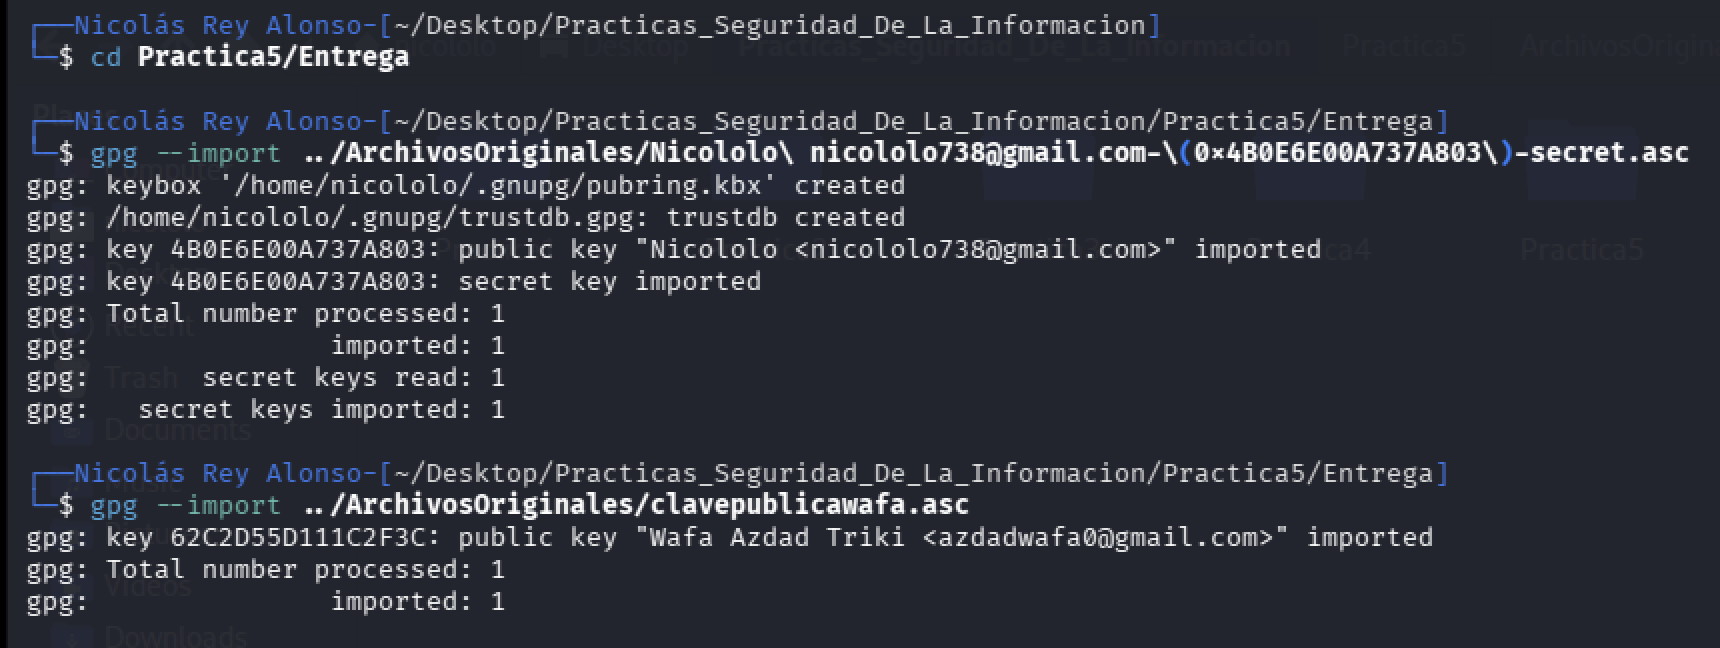
\includegraphics[width=\textwidth]{Imagenes/11-ImportarClavesGNUPGTerminal.png}
    \caption{Importación con \texttt{gpg --import} de la clave pública de Wafa Azdad Triki, mostrando el finguerprint e importación de la ``raíz''}
    \label{fig:importar_clave_publica_y_raiz}
\end{figure}

\section{Paso 3 -- Asignación de confianza máxima a la clave de la compañera}

Inicialmente, al importar la clave de Wafa, GnuPG le asigna un nivel de confianza \textbf{unknown}. Para que la verificación de firma sea completa y no genere advertencias, es necesario asignarle \textbf{confianza máxima (ultimate)}.

Se ejecuta el comando de edición de clave:

\begin{lstlisting}[caption=Asignación de confianza máxima (ultimate) a la clave de Wafa]
gpg --edit-key 62C2D55D111C2F3C
\end{lstlisting}

Dentro del editor interactivo de GnuPG, se sigue la siguiente secuencia:

\begin{enumerate}
    \item \texttt{gpg> trust} --- inicia el modo de asignación de confianza.
    \item GnuPG muestra los niveles disponibles (1 a 5). Se introduce \texttt{5} (\textit{I trust ultimately}).
    \item GnuPG pide confirmación: \textit{Do you really want to set this key to ultimate trust?} Se responde \texttt{y}.
    \item \texttt{gpg> quit} --- sale del editor.
\end{enumerate}

\begin{figure}[H]
    \centering
    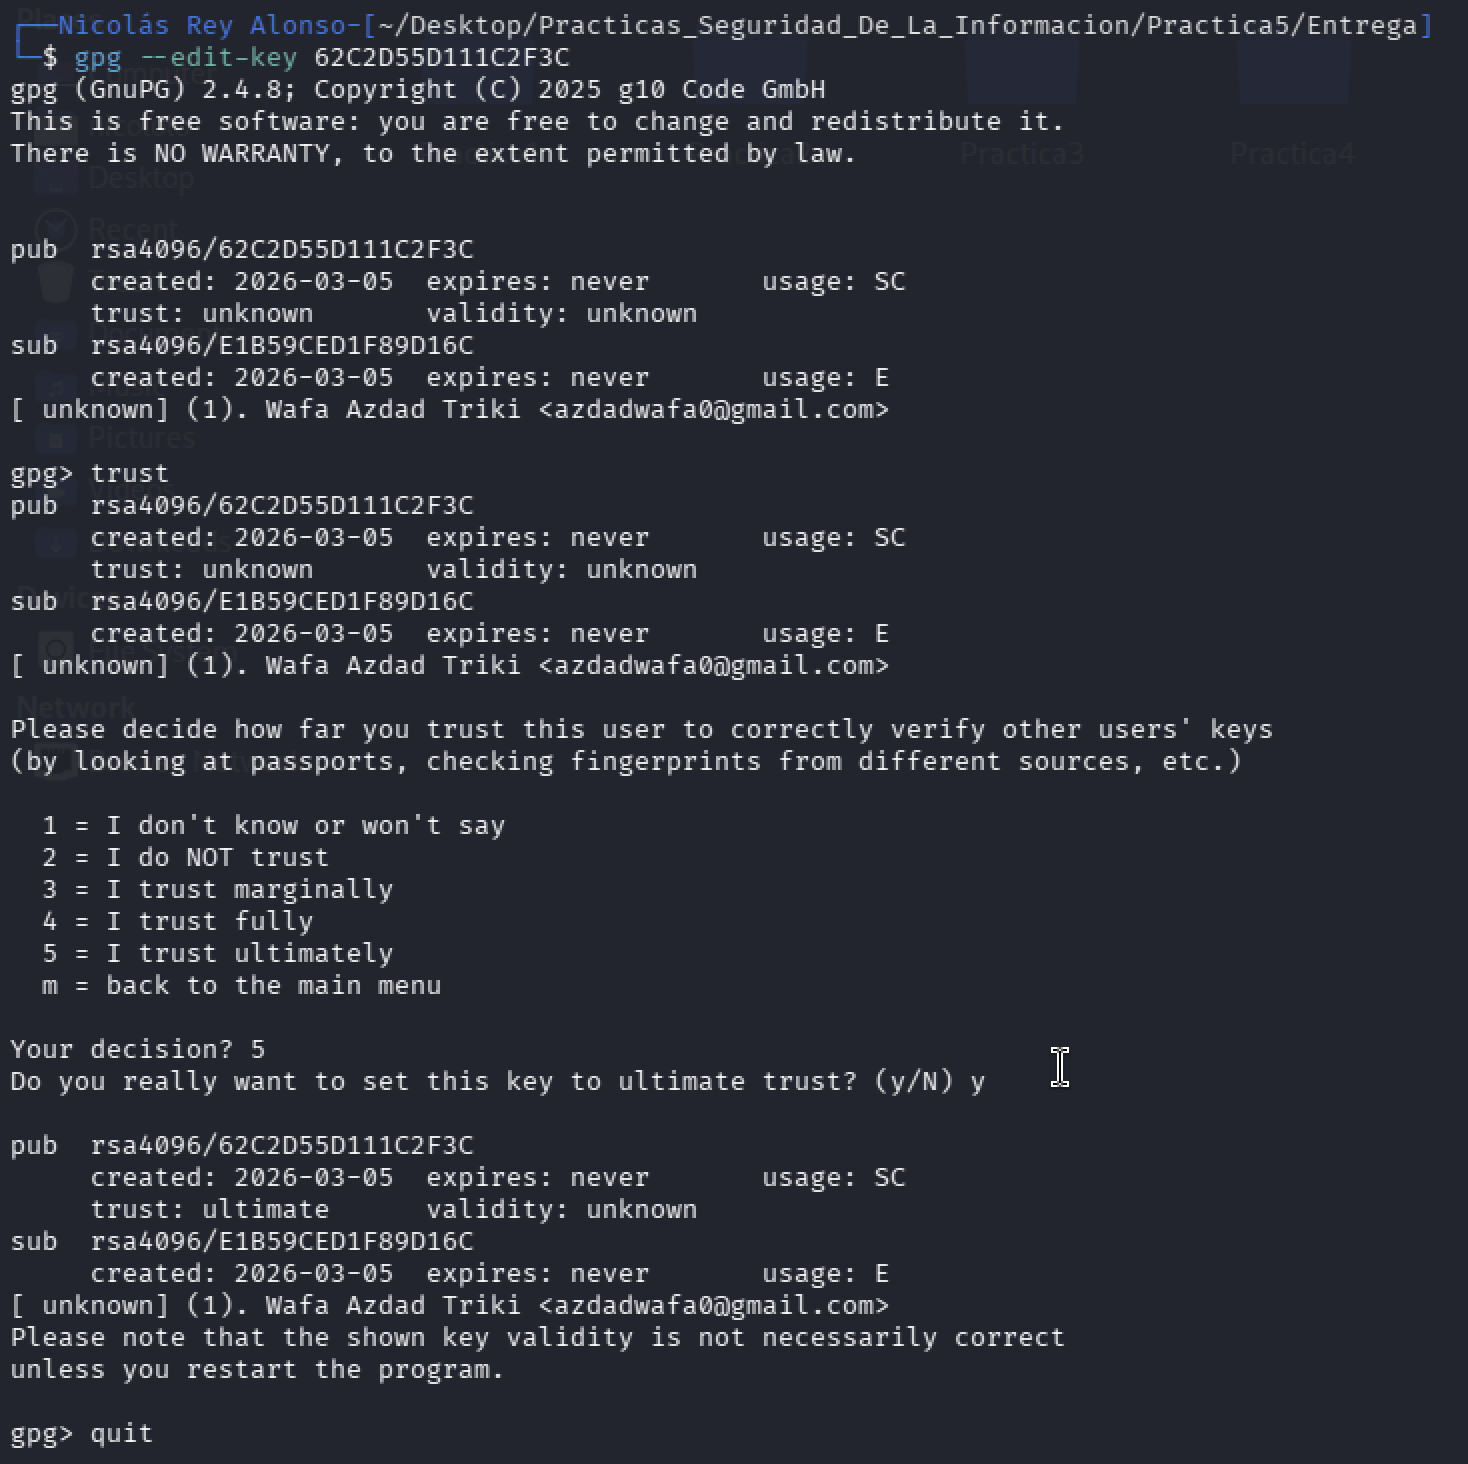
\includegraphics[width=\textwidth]{Imagenes/12-DarConfianzaClaveWafaTerminal.png}
    \caption{Sesión de \texttt{gpg --edit-key} asignando confianza máxima (ultimate) a la clave de Wafa}
    \label{fig:dar_confianza}
\end{figure}

Tras asignar la confianza, el campo \texttt{trust} de la clave pasa de \texttt{unknown} a \texttt{ultimate}. La validez (\texttt{validity}) seguirá apareciendo como \texttt{unknown} hasta reiniciar GnuPG, lo cual es un comportamiento esperado.

\textbf{Nota:} Los niveles de confianza de GnuPG son:
\begin{itemize}[label=\textbullet]
    \item \texttt{1} -- unknown / no sé o no diré
    \item \texttt{2} -- no confío en absoluto
    \item \texttt{3} -- confío marginalmente
    \item \texttt{4} -- confío completamente
    \item \texttt{5} -- confío de forma absoluta (ultimate)
\end{itemize}

\section{Paso 4 -- Descifrado y verificación de la firma}

El comando principal para descifrar un mensaje OpenPGP y verificar su firma simultáneamente es:

\begin{lstlisting}[caption=Descifrado y verificación del mensaje OpenPGP con gpg]
gpg --decrypt ../ArchivosOriginales/Correo_Cifrado.eml \
    > ../Salida/correodescifrado.mime 2>&1
\end{lstlisting}

GnuPG realiza internamente las siguientes operaciones:
\begin{enumerate}
    \item Detecta que el mensaje está cifrado con nuestra subclave de cifrado (\texttt{cv25519}, ID \texttt{B809E1B2EC24D298}).
    \item Descifra el contenido usando nuestra clave privada.
    \item Verifica la firma digital del remitente usando la clave pública de Wafa.
\end{enumerate}

La salida muestra información de diagnóstico en \texttt{stderr} y el contenido descifrado en \texttt{stdout}. Redirigiendo ambas al mismo fichero con \texttt{2>\&1} obtenemos un archivo de texto que incluye:

\begin{itemize}[label=\textbullet]
    \item Las líneas de diagnóstico de gpg (claves usadas para cifrado, resultado de la verificación).
    \item Las cabeceras MIME del mensaje descifrado (\texttt{Content-Type}, \texttt{Subject}, \texttt{From}, \texttt{To}, etc.).
    \item El cuerpo del mensaje en texto plano: \textit{``Firmado y cifrado''}.
    \item La clave pública de Wafa adjunta en formato PGP ARMORED.
\end{itemize}

\begin{figure}[H]
    \centering
    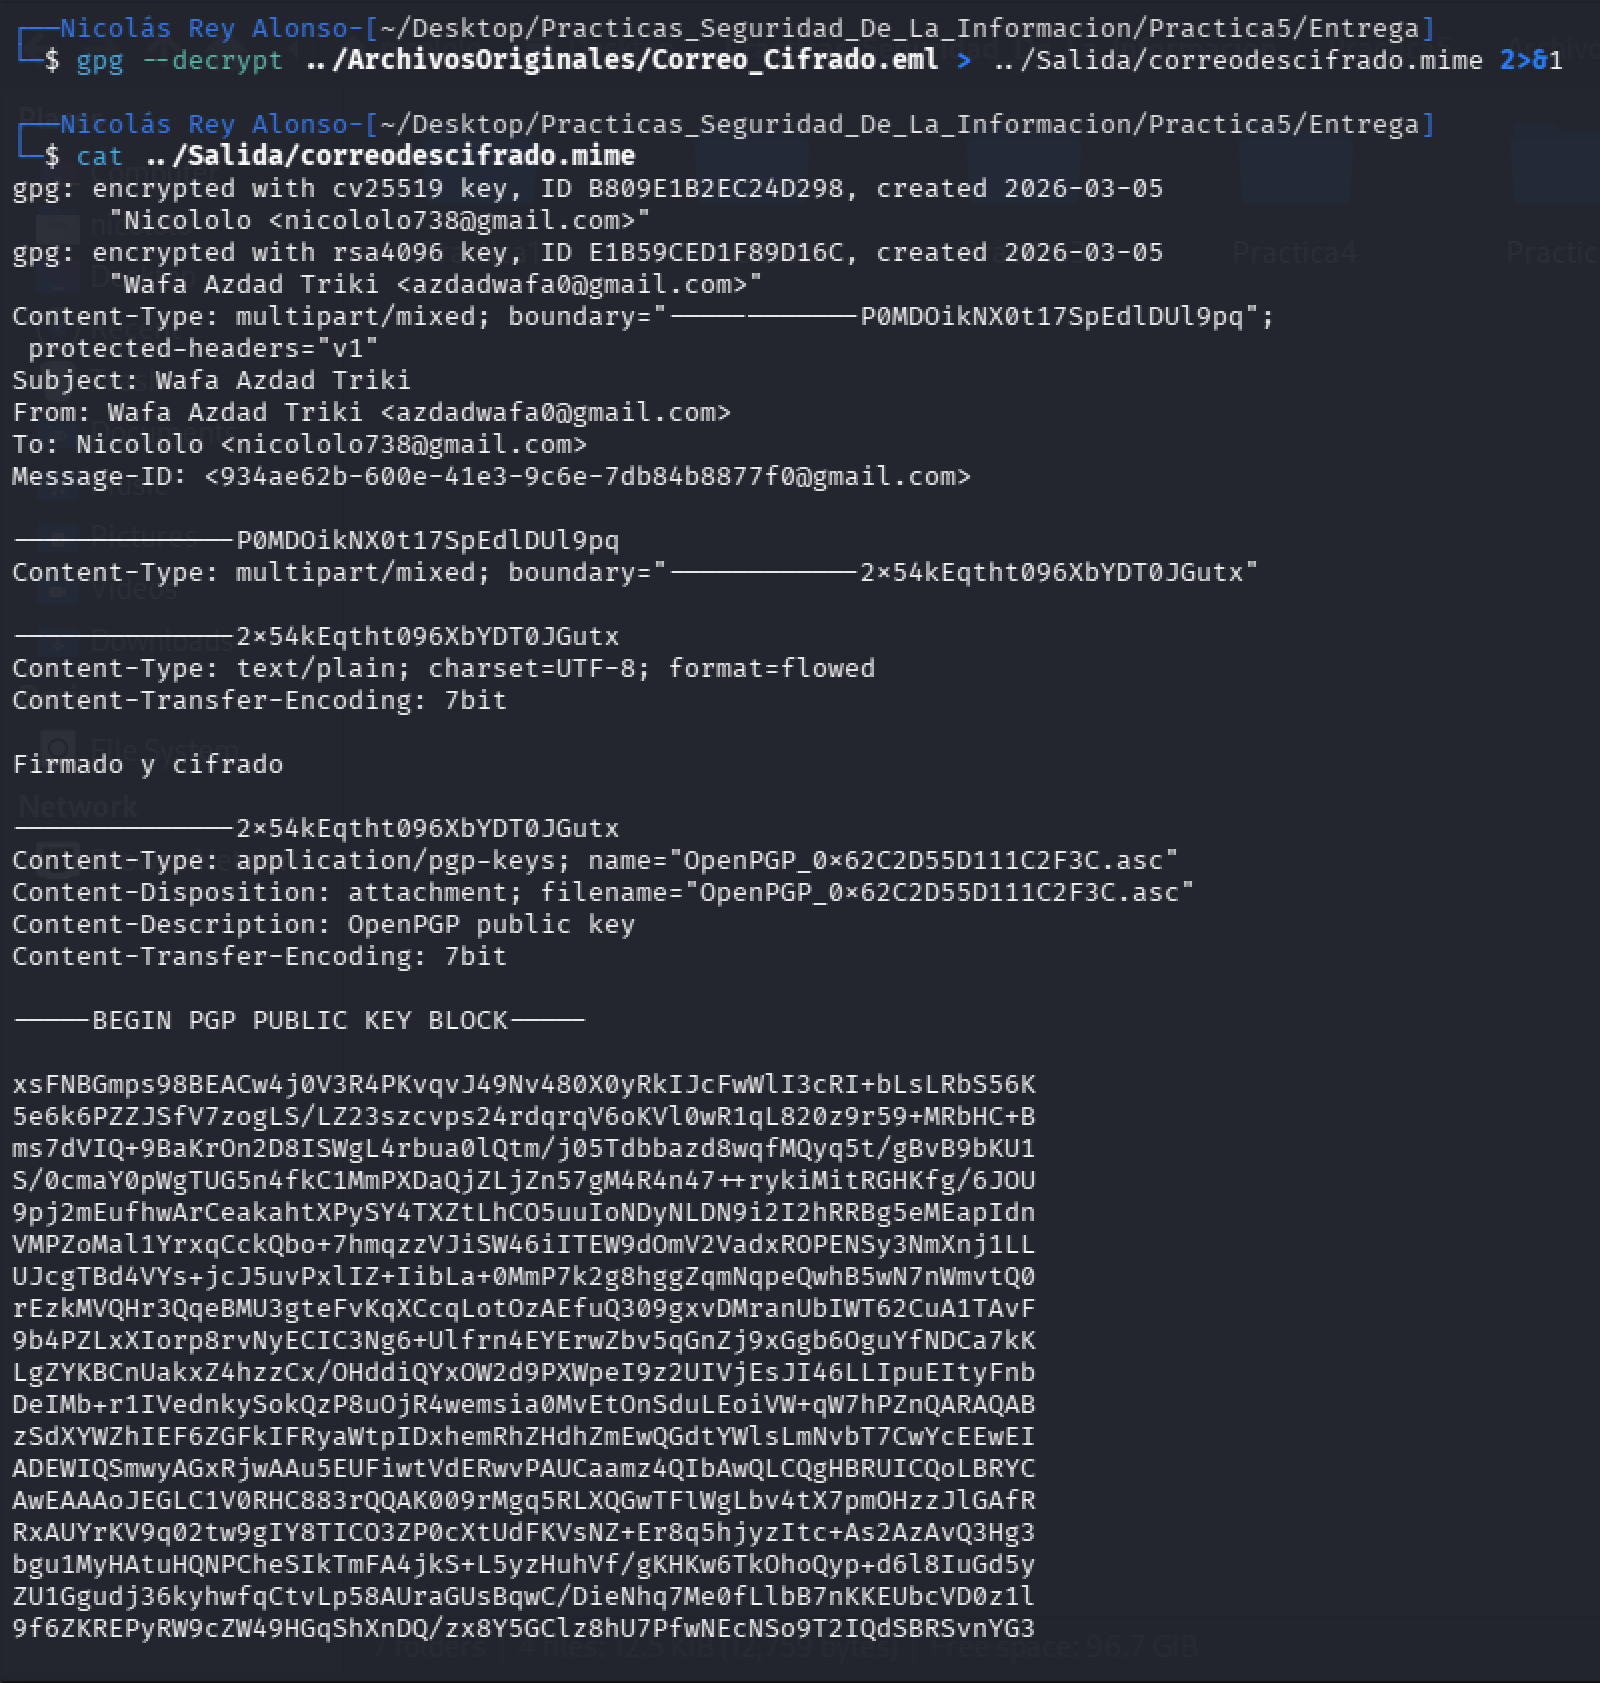
\includegraphics[width=\textwidth]{Imagenes/13-DesencriptarMensajeOpenPGP.png}
    \caption{Salida del comando \texttt{gpg --decrypt} mostrando el mensaje descifrado y la estructura MIME}
    \label{fig:descifrar_mensaje}
\end{figure}

\subsection{Análisis de la salida}

Las primeras líneas del fichero descifrado muestran los metadatos del descifrado:

\begin{lstlisting}[caption=Cabeceras de diagnóstico de gpg en la salida descifrada]
gpg: encrypted with cv25519 key, ID B809E1B2EC24D298, created 2026-03-05
     "Nicololo <nicololo738@gmail.com>"
gpg: encrypted with rsa4096 key, ID E1B59CED1F89D16C, created 2026-03-05
     "Wafa Azdad Triki <azdadwafa0@gmail.com>"
\end{lstlisting}

Esto confirma que el mensaje fue cifrado para \textbf{dos destinatarios}: nuestra subclave de cifrado y la de Wafa (la remitente se incluyó a sí misma como destinataria para poder leer el mensaje enviado).

A continuación, el contenido MIME descifrado incluye las cabeceras del mensaje:

\begin{lstlisting}[caption=Cabeceras MIME del mensaje descifrado]
Content-Type: multipart/mixed; boundary="...P0MDOikNX0t17SpEdlDUl9pq"
Subject: Wafa Azdad Triki
From: Wafa Azdad Triki <azdadwafa0@gmail.com>
To: Nicololo <nicololo738@gmail.com>
\end{lstlisting}

Y el cuerpo de texto plano:

\begin{lstlisting}[caption=Cuerpo del mensaje descifrado]
Content-Type: text/plain; charset=UTF-8; format=flowed
Content-Transfer-Encoding: 7bit

Firmado y cifrado
\end{lstlisting}

\section{Paso 5 -- Extracción de adjuntos MIME con ripmime}

Dado que el mensaje descifrado contiene cabeceras MIME, si se quiere extraer cada parte por separado (texto, clave pública adjunta, etc.) se puede usar la utilidad \textbf{ripmime}:

\begin{lstlisting}[caption=Extracción de adjuntos MIME con ripmime]
gpg --decrypt mensaje.eml > mensaje.mime
mkdir dir_final
ripmime mensaje.mime dir_final
\end{lstlisting}

Esto crearía en \texttt{dir\_final/} un fichero de texto con el cuerpo y otro \texttt{.asc} con la clave pública de Wafa adjunta en el mensaje.

\section{Resumen del flujo completo}

\begin{table}[H]
    \centering
    \caption{Comandos utilizados en la decodificación manual con GnuPG}
    \begin{tabularx}{\textwidth}{c|l|X}
        \toprule
        \textbf{Paso} & \textbf{Comando} & \textbf{Descripción} \\
        \midrule
        1 & \texttt{gpg --import claveprivada.asc} & Importa nuestra clave privada \\
        2 & \texttt{gpg --import clave.asc} & Importa la clave pública de Wafa \\
        3 & \texttt{gpg --edit-key \ldots} $\rightarrow$ trust $\rightarrow$ 5 & Confianza máxima a la clave de Wafa \\
        4 & \texttt{gpg --decrypt mensaje.eml} & Descifra y verifica la firma a la vez \\
        5 & \texttt{ripmime mensaje.mime dir/} & Extrae adjuntos MIME (opcional) \\
        \bottomrule
    \end{tabularx}
\end{table}

A diferencia de S/MIME donde \texttt{openssl smime} requería dos comandos separados (descifrar + verificar), \textbf{GnuPG realiza ambas operaciones en un único paso} con \texttt{gpg --decrypt}, lo que simplifica notablemente el proceso.
